\subsubsection{Diagramma delle classi}
Di seguito è riportato un esempio di diagramma delle classi. Esso rappresenta come è composta la pagina della dashboard\ped{G} e come vengono gestiti i vari component presentational e container.\\ È stata  modificata leggermente la sintassi standard UML\ped{G} per i diagrammi delle classi, in modo da esplicitare la distinzione dei due tipi di component: rettangolo normale per i container, rettangolo con angoli curvati per i presentational.

\vspace{1cm}

\begin{figure}[H]
\centering
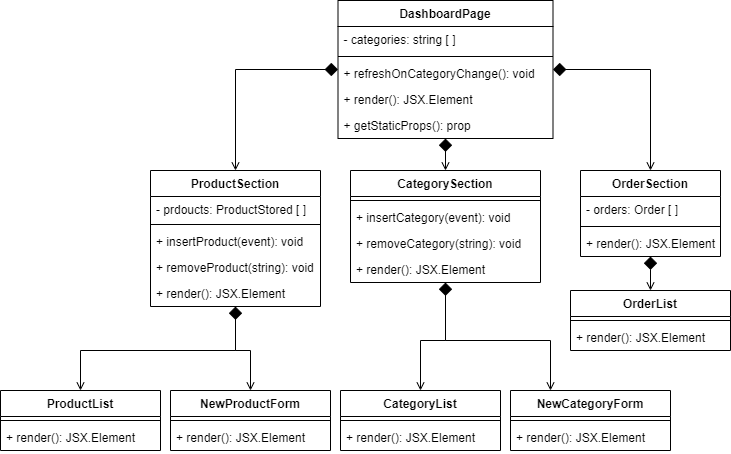
\includegraphics[scale=0.55]{res/Architettura/Frontend/img/class_frontend_dashboard}\\
\caption{Diagramma delle classi della pagina dashboard\ped{G} per il modulo Front-end\ped{G}}
\end{figure}

Viene inoltre mostrato il diagramma per i diversi tipi utilizzati dal nostro modulo.

\begin{figure}[H]
\centering
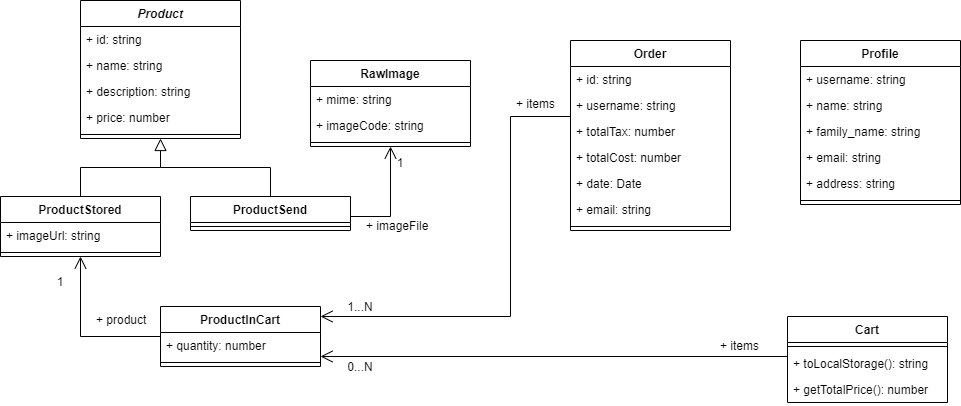
\includegraphics[scale=0.45]{res/Architettura/Frontend/img/class_frontend_types}\\
\caption{Diagramma delle classi dei tipi utilizzati per il modulo Front-end\ped{G}}
\end{figure}